\documentclass[aspectratio=169]{beamer}
\usetheme{Madrid}
\usecolortheme{default}

\usepackage[T1]{fontenc}
\usepackage{lmodern}
\usepackage{graphicx}
\usepackage{tikz}
\usepackage{pgfplots}
\pgfplotsset{compat=1.14}
\usepackage{anyfontsize}
\usepackage{xspace}
\usepackage{amsmath}
\usepackage{booktabs}
\usepackage{caption}
\usepackage{algpseudocode}
\usepackage{hyperref}
\usepackage{graphicx}
\newcommand{\cev}[1]{\reflectbox{\ensuremath{\vec{\reflectbox{\ensuremath{#1}}}}}}


\title[Week 1]
{Score-Based Multimodal Autoencoders}

\subtitle{Week 12}

\author[] % (optional, for multiple authors)
{
Konstantin Yakovlev \inst{1} \and
}

\institute[] % (optional)
{
  \inst{1}%
  MIPT \\
  Moscow, Russia
}

\date[MIPT 2023] % (optional)
{MIPT 2023}

% \logo{\includegraphics[height=0.8cm]{logo_uoft}}

\definecolor{uoftblue}{RGB}{6,41,88}
\setbeamercolor{titlelike}{bg=uoftblue}
\setbeamerfont{title}{series=\bfseries}

\begin{document}

\frame{\titlepage}


\begin{frame}{Score-Based Multimodal Autoencoders\footnote{\href{https://arxiv.org/pdf/2305.15708.pdf}{Wesego D. et. al, Score-Based Multimodal Autoencoders, 2023}}}
    \begin{minipage}{0.49\textwidth}
        \textbf{Challenge}: conditioning on more modalities often reduces the quality of the generated modality. \\
        \textbf{Solution}: instead of learning a joint posterior, try to model a joint prior $p_\theta(\mathbf{z}_{1:M})$.
        This allows us to better model correlation among modalities. \\
        \textbf{The Method}: Assume that
        \begin{small}
        \begin{align*}
            &p(\mathbf{x}_{1:M}|\mathbf{z}_{1:M}) = \prod_{k=1}^Mp(\mathbf{x}_k|\mathbf{z}_k), \\
            &q(\mathbf{z}_{1:M}|\mathbf{x}_{1:M}) = \prod_{k=1}^Mq(\mathbf{z}_k|\mathbf{x}_k).
        \end{align*}
        \end{small}
        Then, $\mathrm{ELBO} = \sum_k\mathrm{ELBO}_k$ if the prior is decomposable.
    \end{minipage}
    \begin{minipage}{0.49\textwidth}
        \textbf{Two-stage training}:
        \begin{itemize}
            \item Train the autoencoders separately, assuming that $p(\mathbf{z}_m) = \mathcal{N}(0, \mathbf{I})$.
            \item Freeze the autoencoders and leran a joint prior $p(\mathbf{z}_{1:M})$.
            More precisely, we need a score function $s_\theta(\mathbf{z}_{1:M})$ to sample from the prior.
        \end{itemize}
        Finally, it becomes trivial to sample from any subset of missing modalities using Langevin dynamics.
    \end{minipage}
\end{frame}


\begin{frame}{Dimension reduction via score ratio matching\footnote{\href{https://openreview.net/pdf?id=YAN97j2NmGT}{Baptista R. et. al, Dimension reduction via score ratio matching, 2022}}}
    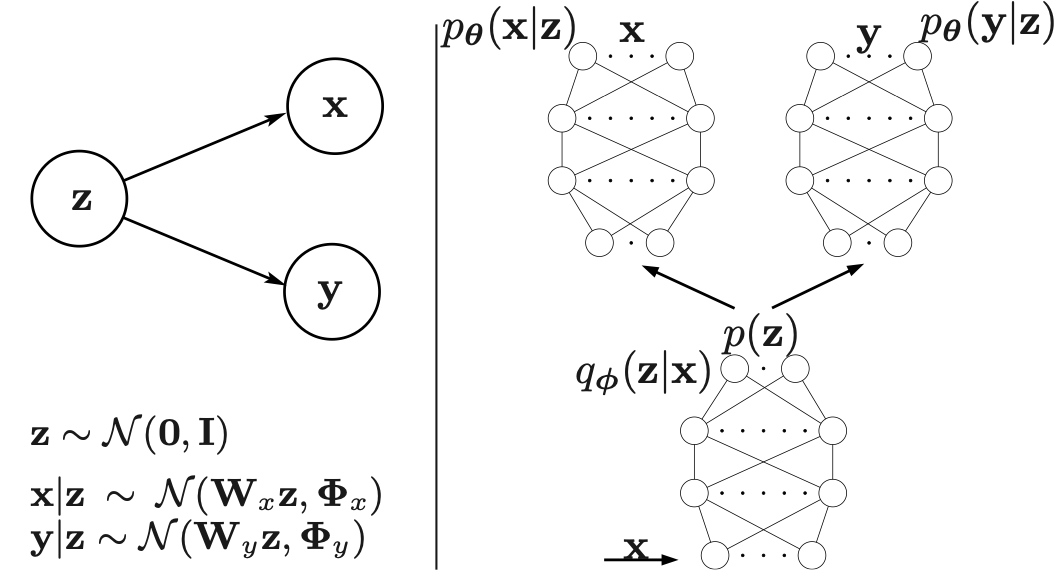
\includegraphics[width=\textwidth]{figures/fig1.png}
    \begin{align*}
        \pi_r(\mathbf{x}) \propto f(\mathbf{U}_r^\top \mathbf{x})\rho(\mathbf{x}).
    \end{align*}
    \textbf{Proposition}: $D_\text{KL}(\pi||\pi_r) \leq \frac{1}{2}(\lambda_{r + 1} + \ldots + \lambda_d)$.
\end{frame}


\begin{frame}{Learning the correlation among the latent variables (proposed)}
    \textbf{Challenge}: Score-Based Multimodal Autoencoders do not select the dimension of the latent
    space of each modality properly. Therefore, this makes it more difficult to learn correlations among the
    modalities. \\
    \textbf{Solution}: reduce the dimension of the latent space of each modality.
    \begin{align*}
        \pi_r(\mathbf{x}_{1:M}) \propto f(\mathbf{W}^\top\mathbf{x}_{1:M})\prod_{m=1}^M\rho(\mathbf{x}_m), \quad
        \mathbf{W}^\top = \mathrm{diag}(\mathbf{U}_1^\top, \ldots, \mathbf{U}_M^\top).
    \end{align*}
    \textbf{Proposition}: the proposed parametrization does not require an additional computational cost
    when computing the eigenpairs of $\mathbf{H}$. \\
    \textbf{Note}: other modalities $\mathbf{x}_{\setminus m}$ contribute to the reduction of the dimension of
    the modality $\mathbf{x}_m$.

\end{frame}


\begin{frame}{Project description}
    \textbf{Title}: Learning the correlation among modalities. \\
    \textbf{Problem}: Consider a multimodel generative modeling task. The goal of inference is to sample unobserved modalities
    given the observed ones. The challenge is that Score-Based Multimodal Autoencoders do not select the dimension of the latent
    space of each modality properly. Therefore, this makes it more difficult to learn correlations among the
    modalities.\\
    \textbf{Data}: \href{https://openreview.net/forum?id=5Y21V0RDBV}{PolyMnist},
    \href{https://openaccess.thecvf.com/content_CVPR_2020/papers/Lee_MaskGAN_Towards_Diverse_and_Interactive_Facial_Image_Manipulation_CVPR_2020_paper.pdf}{CelebAMask-HQ}. \\
    \textbf{Reference}: (1) and (2). \\
    \textbf{Basic solution}: Score-Based Multimodal AE: instead of learning a joint posterior,
     model a joint prior. This allows us to better capture the correlations among modalities. \\
    \textbf{Proposed solution}: Reduce the dimension of the latent space of each modality with Score Ratio Matching. \\
    \textbf{Novelty}: we address the challenge of generative quality degradation when the number of modalities increases.
\end{frame}


\end{document}